\documentclass[preprintnumbers,amsmath,amssymb,onecolumn,12pt]{revtex4-2}
\usepackage{graphicx}% Include figure files
\usepackage{dcolumn}% Align table columns on decimal point
\usepackage{bm}% bold math
\usepackage{natbib}
\usepackage{physics}
\usepackage[caption=false]{subfig}
\newcommand{\be}{\begin{equation}}
\newcommand{\ee}{\end{equation}}

\newcommand{\bea}{\begin{eqnarray}}
\newcommand{\eea}{\end{eqnarray}}
 
\def\sgn{\mathop{\rm sgn}}

\begin{document}
\vspace{0.2in}
{\Large \hspace{1.6in}\textsc{Supplementary Material} }\\
\
\title{Low field depolarization of electronic spins through dipole-dipole coupling}

\author{C. Pellet-Mary$^1$, M. Perdriat$^1$, G. H\'etet$^1$} 

\affiliation{Laboratoire De Physique de l'\'Ecole Normale Sup\'erieure, \'Ecole Normale Sup\'erieure, PSL Research University, CNRS, Sorbonne Universit\'e, Universit\'e Paris Cit\'e , 24 rue Lhomond, 75231 Paris Cedex 05, France.}

\maketitle

\tableofcontents

\section{NV Hamiltonian}
\section{Samples}
\section{Experimental Setup}
\section{Data analysis}
\subsection{$T_1$ fitting Protocol}
\begin{figure}
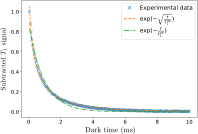
\includegraphics[width=0.8\textwidth]{Figures_SI/Fig_T1_0B}
\caption{$T_1$ measurement in zero magnetic field with purely exponential and purely stretched exponential fits}
\label{T1_0B}
\end{figure}
\begin{figure}
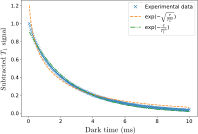
\includegraphics[width=0.8\textwidth]{Figures_SI/Fig_T1_1x1x1x1}
\caption{$T_1$ measurement in non-zero magnetic field with purely exponential and purely stretched exponential fits}
\label{T1_1x4}
\end{figure}
\begin{figure}
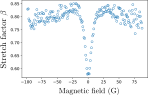
\includegraphics[width=0.45\textwidth]{Figures_SI/fig_alphas}
\caption{Best stretch factor $\beta$ for a $T_1$ fit of the form $f(\tau)=A \exp(-(\frac{\tau}{T_1})^\beta)$}
\label{alphas}
\end{figure}
\subsection{Estimation of fluctuators width}
\section{Les détails qui tuent}
\subsection{Effect of laser polarization}
\begin{figure}
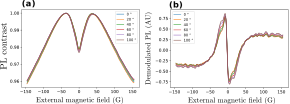
\includegraphics[width=0.9\textwidth]{Figures_SI/fig_Pola}
\caption{Effect of the polarization of the incident laser. (a) Photoluminescence as a function of randomly oriented magnetic field for various polarization angle. (b) Demodulated PL in the same conditions}
\label{Pola}
\end{figure}
\subsection{Alignment of B}
La faudrait p-e montrer ce qu'il se passe pour un décalage de quelques degrés. A voir si j'ai déja les plots
\section{Fluctuator et tout}
\subsection{121 VS 22}
\subsection{100 vs 0B}

\bibliographystyle{plain}
\bibliography{CR_SI}{}
\end{document}